Our preliminary evaluation demonstrates that this approach shows a lot of
promise, however the software and hardware still need to be tuned in order to
better decide which keys to accelerate.

\subsection{Methodology}

In our experimental setup, we generated keys, put all of them in memcached and
then did a GET request for all of the keys in turn. We then measured the
latencies for all of the GET requests of the keys we put in the accelerator.
There were multiple distributions that we used in order to exercise our system.

\subsection{Results}

Initially, we looked at how our system does against a software implementation.
In this experiment, we put a key on the accelerator and a key in the unmodified
software implementation of memcached. We then issued many GET requests and
recorded the latency of all requests. In between GET requests, we sometimes had
a small inter-arrival time, which also varied according to our sample
distributions.

\begin{figure}[t]
\begin{center}
\label{fig:one-req}
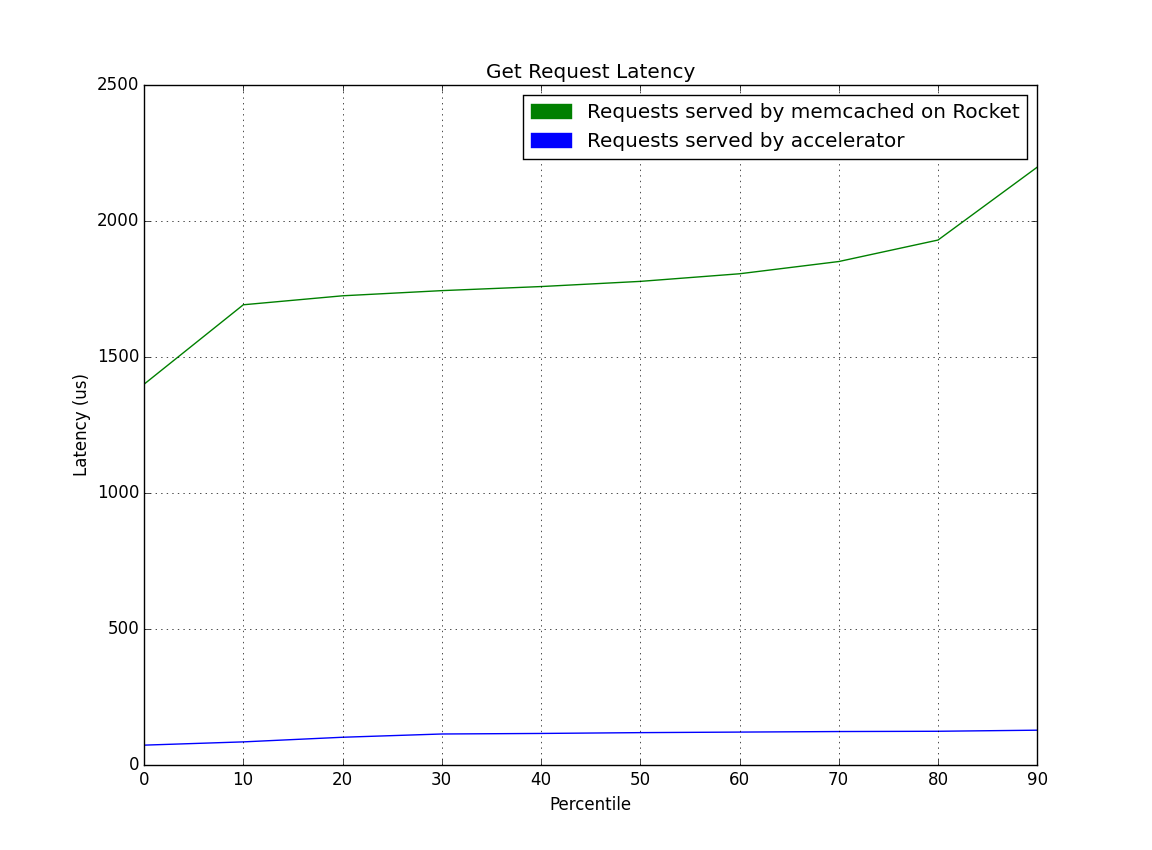
\includegraphics[width=\linewidth]{graph.png}
\caption{Latency of GET requests when only getting 1 key}
\end{center}
\end{figure}

\begin{figure}[t]
\begin{center}
\label{fig:unif}
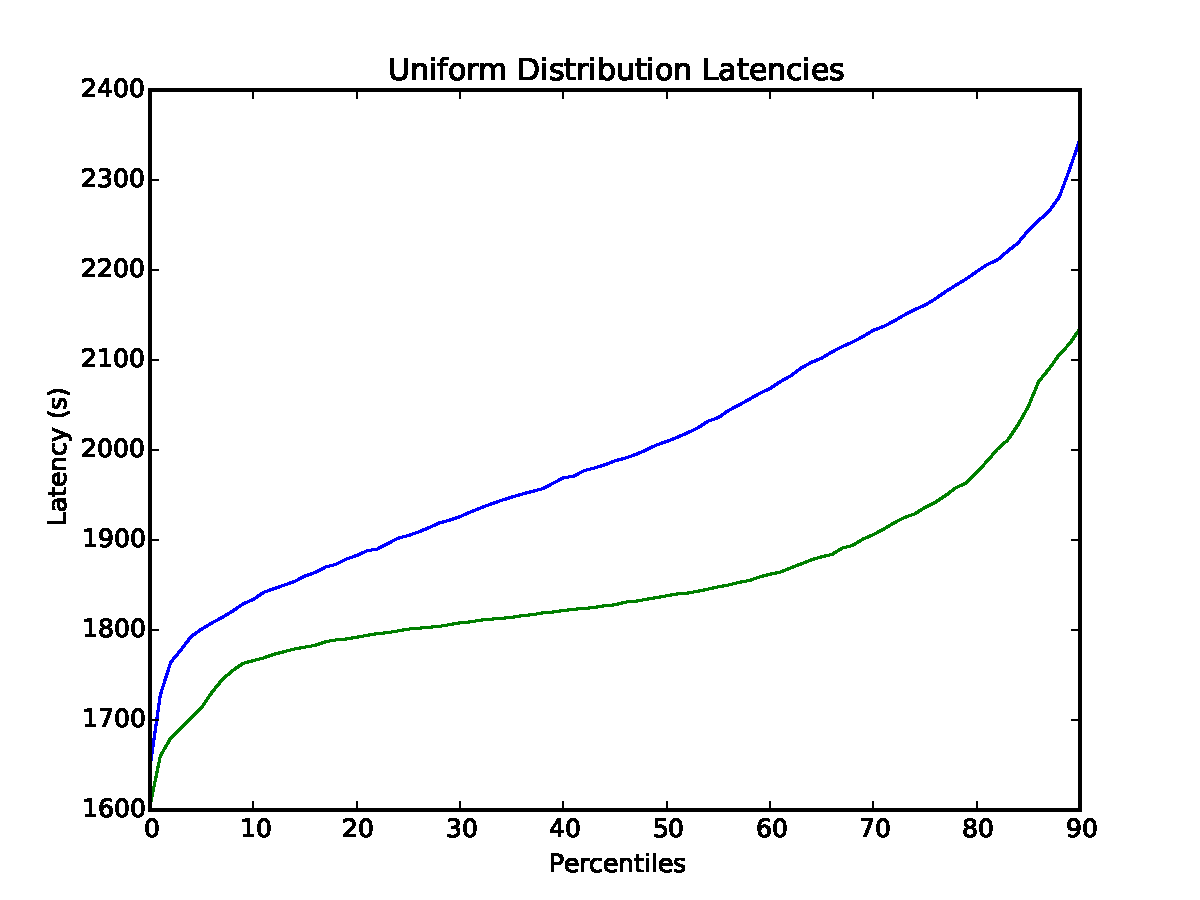
\includegraphics[width=\linewidth]{unif.pdf}
\caption{Latency of GET requests when keys follow a uniform distribution}
\end{center}
\end{figure}

\begin{figure}[t]
\begin{center}
\label{fig:norm}
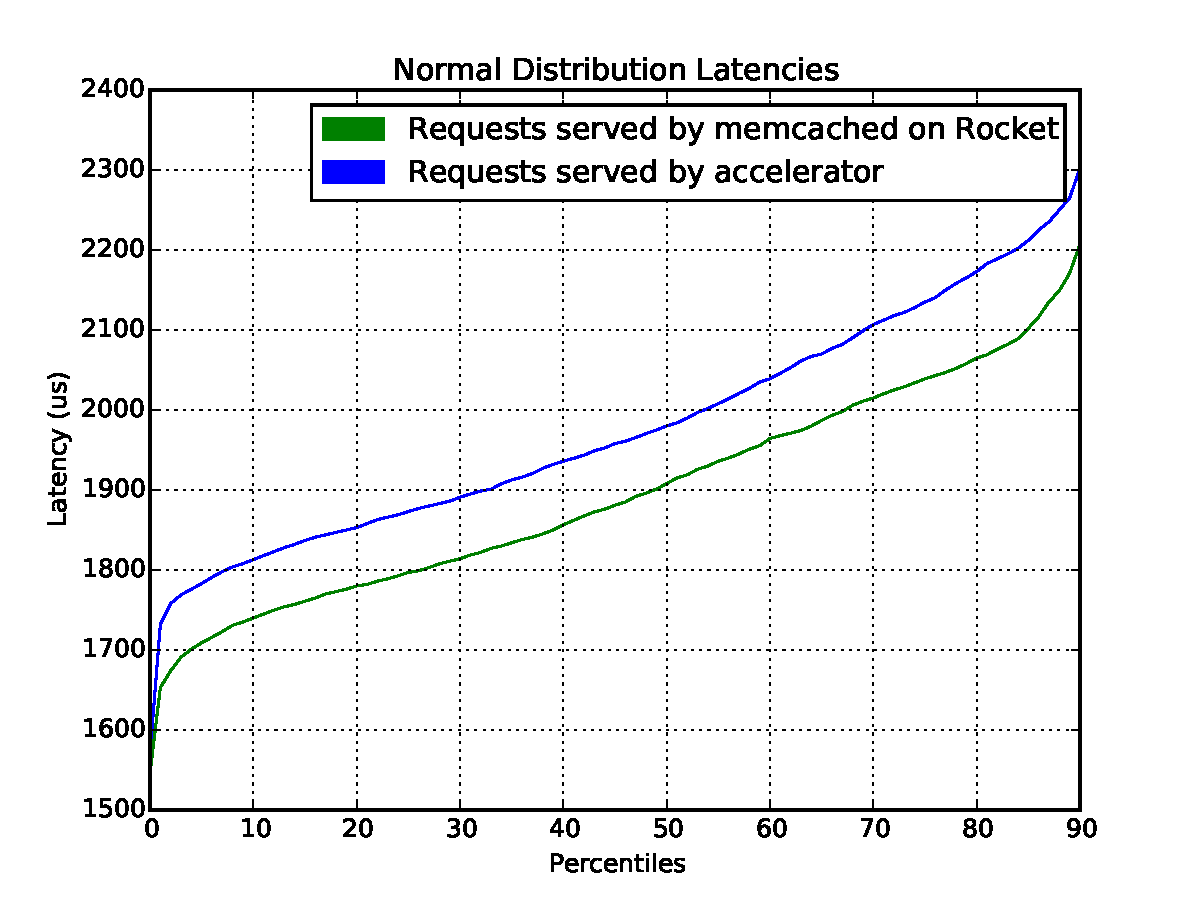
\includegraphics[width=\linewidth]{norm.pdf}
\caption{Latency of GET requests when keys follow a normal distribution}
\end{center}
\end{figure}

As we see from Figure \ref{fig:one-req}, there is approximately an order of magnitude
improvement when a key is in the accelerator compared to the key being returned
from the CPU running memcached.

Furthermore, in order to exercise our accelerator fully, we used a bunch of
synthetically generated distributions for the keys. In Figure \ref{fig:unif},
we ran it on a uniform distribution of keys. We see that in this distribution,
the software driven accelerator does worse than than the pure software
implementation. The driving factor behind the poor performance is the overhead
incurred from the filter when processing each key to check if it is already in
the accelerator. Thus, these distributions do not leverage the benefits of the
hardware cache while paying the penalty of the filter. Therefore, the poor
performance of distributions that are not highly skewed is to be expected from
our design. In fact, the results shown in Figure \ref{fig:norm} corroborate
these results since the unmodified software implementation outperforms our
system.

\begin{figure}[t]
\begin{center}
\label{fig:pareto}
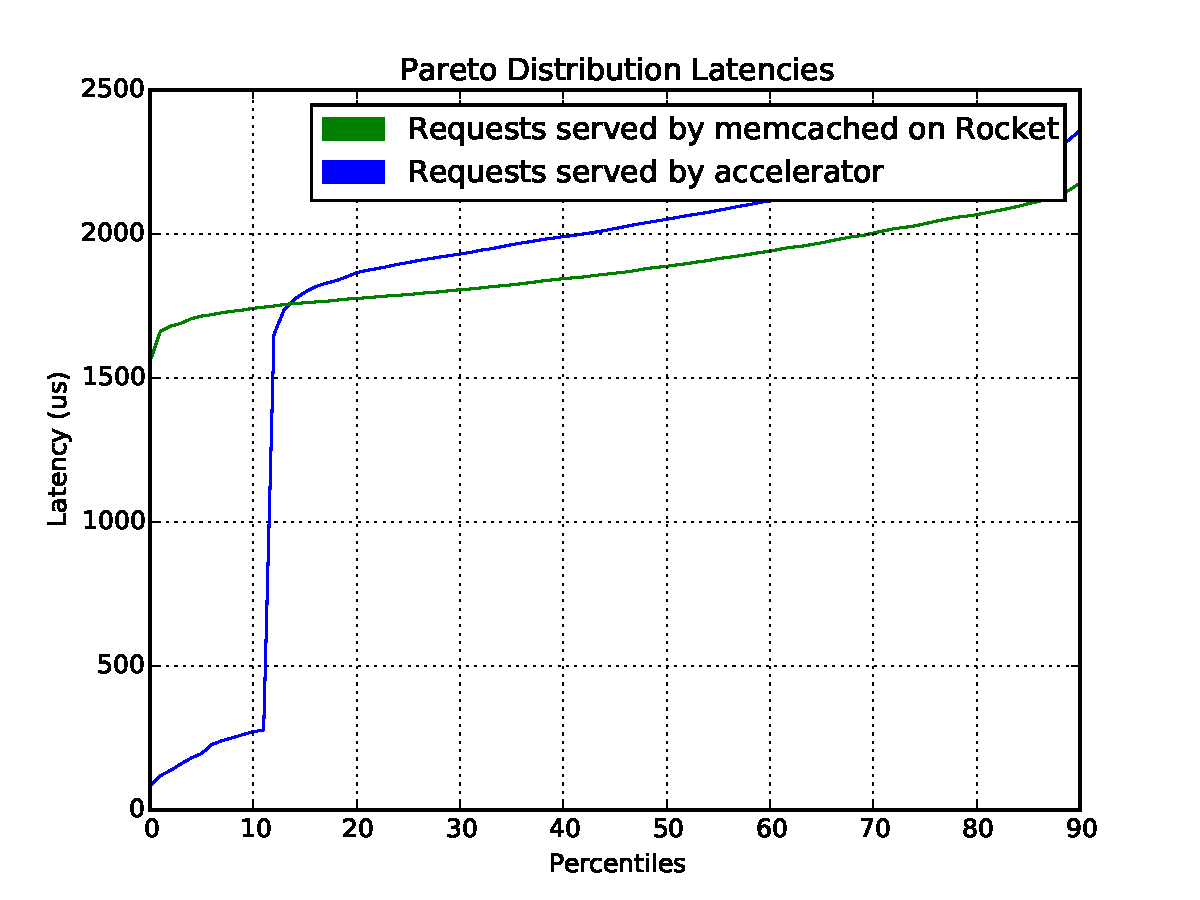
\includegraphics[width=\linewidth]{pareto.pdf}
\caption{Latency of GET requests when keys follow a pareto distribution}
\end{center}
\end{figure}

\begin{figure}[t]
\begin{center}
\label{fig:etc}
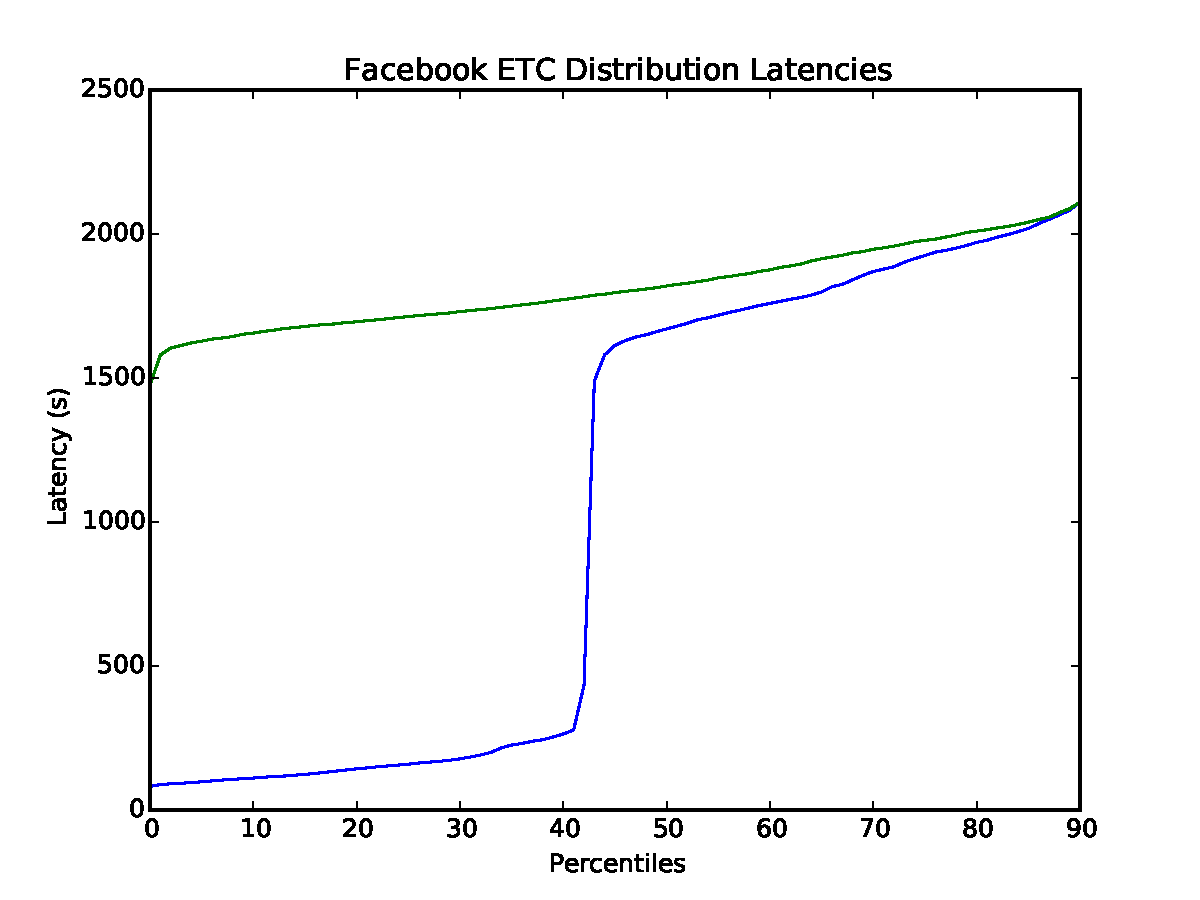
\includegraphics[width=\linewidth]{etc.pdf}
\caption{Latency of GET requests when keys follow the Facebook ETC distribution}
\end{center}
\end{figure}

For skewed distributions, we see that the benefits of accelerating a small
fraction of the keys is quite large. On our synthetically generated pareto
distribution in Figure \ref{fig:pareto}, we see that the highly skewed keys get the
benefit of a $10$ times improvement over the software implementation. This is
due to the fact that once a hot key gets on the accelerator, it is very hard
for it to get kicked out unless it becomes cold. This is because if it was to
be kicked out by another key, then that key must have been hotter. However, for
highly skewed distributions, the probabilty of two hot keys having a cache
collision is very small. In addition, we see that the software managed
accelerator actually increases the latency for a bunch of keys as well. This is
due to the fact that there is a filter as well, so we are incurring a small
overhead for a large portion of the keys.

Finally, we used the Facebook ETC distribution~\cite{AXFJP2012} in order to see
how our system would fare against a real life workload. In Figure
\ref{fig:etc}, we see that this is a very promising start. $40$ percent of all
requests get a $10$ times improvement in latencies. However, our synthetic
workloads suggest that there are some improvements to be made in our caching
policy that will probably enhance the performance of our system as well.
